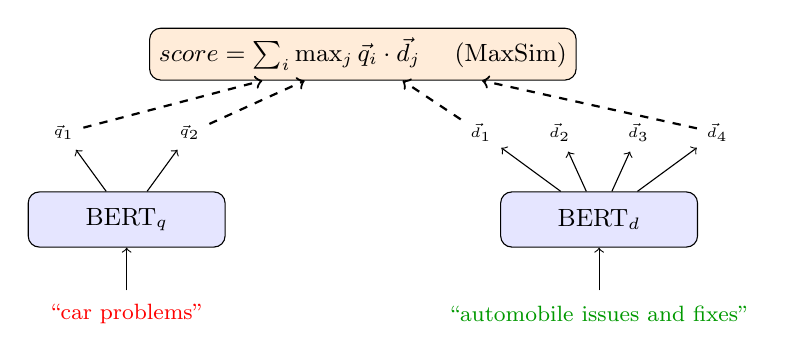
\begin{tikzpicture}[
    box/.style={rectangle, draw, rounded corners, fill=blue!10, minimum height=0.7cm, align=center, font=\small},
    arrow/.style={->, thick}
]
    \node[box, minimum width=2.5cm] (bq) at (0, 1.5) {BERT$_q$};
    \node[box, minimum width=2.5cm] (bd) at (6, 1.5) {BERT$_d$};

    \node[font=\footnotesize, red] at (0, 0.3) {``car problems''};
    \node[font=\footnotesize, green!60!black] at (6, 0.3) {``automobile issues and fixes''};

    \node[font=\tiny] (e1) at (-0.8, 2.6) {$\vec{q}_1$};
    \node[font=\tiny] (e2) at (0.8, 2.6) {$\vec{q}_2$};

    \node[font=\tiny] (d1) at (4.5, 2.6) {$\vec{d}_1$};
    \node[font=\tiny] (d2) at (5.5, 2.6) {$\vec{d}_2$};
    \node[font=\tiny] (d3) at (6.5, 2.6) {$\vec{d}_3$};
    \node[font=\tiny] (d4) at (7.5, 2.6) {$\vec{d}_4$};

    \draw[arrow, thin] (0, 0.6) -- (bq);
    \draw[arrow, thin] (6, 0.6) -- (bd);

    \draw[arrow, thin] (bq) -- (e1);
    \draw[arrow, thin] (bq) -- (e2);
    \draw[arrow, thin] (bd) -- (d1);
    \draw[arrow, thin] (bd) -- (d2);
    \draw[arrow, thin] (bd) -- (d3);
    \draw[arrow, thin] (bd) -- (d4);

    \node[rectangle, draw, fill=orange!15, rounded corners, font=\small] (maxsim) at (3, 3.6) {$\text{score} = \sum_i \max_j \vec{q}_i \cdot \vec{d}_j$ \quad (MaxSim)};

    \draw[arrow, dashed] (e1) -- (maxsim);
    \draw[arrow, dashed] (e2) -- (maxsim);
    \draw[arrow, dashed] (d1) -- (maxsim);
    \draw[arrow, dashed] (d4) -- (maxsim);
\end{tikzpicture}
